\chapter{Interest rate theory}

\section{Zero Coupon Bonds and interest rates}

\begin{definition}[\textbf{Zero Coupon Bond} \cite{filipovic2009term}]
A zero coupon bond (T-bond) with a maturity $T$ guarantees the holder one dollar to be paid out at maturity $T$. We denote the time $t$ price of the zero coupon bond as $P(t,T)$
\end{definition}

We will assume the following: 
\begin{itemize}
    \item There is a frictionless market for $T$-bonds for all $T>0$
    \item $P(T,T) = 1$ for all $T$
    \item $P(t,T)$ is differentiable in $T$.
\end{itemize} 

\begin{tikzpicture}[snake=zigzag, line before snake = 5mm, line after snake = 5mm]
    % draw horizontal line   
    \draw (0,0) -- (4,0);
    
    % draw vertical lines
    \foreach \x in {0,1,2,3,4}
      \draw (\x cm,3pt) -- (\x cm,-3pt);

    % draw nodes
    \draw (0,0) node[below=3pt] {$ 0 $} node[above=3pt] {$   $};
    \draw (1,0) node[below=3pt] {$ S $} node[above=3pt] {$  $};
    \draw (2,0) node[below=3pt] {$ t $} node[above=3pt] {$  $};
    \draw (3,0) node[below=3pt] {$ T $} node[above=3pt] {$  $};
  \end{tikzpicture}

\begin{definition}[\textbf{Simple forward rate \cite{filipovic2009term}}]
The simple forward rate for $[S,T]$ prevailing at time $t\leq T$
is defined as: 
\begin{equation*}
F(t,S,T) = \frac{1}{T-S}\frac{P(t,S)-P(t,T)}{P(t,T)}    
\end{equation*}
\end{definition}

\begin{definition}[\textbf{Continuously compounding forward rate \cite{filipovic2009term}}]
The continuously compounded forward rate for $[S,T]$ prevailing at $t\leq T$ is given by:
\begin{equation*}
    R(t;S,T) = -\frac{\ln{P(t,T)}-\ln{P(t,S)}}{T-S}
\end{equation*}    
\end{definition}

\begin{definition}[\textbf{Instantaneous forward rate \cite{filipovic2009term}}]
The instantaneous forward rate with maturity $T$, prevailing at time $t$ is defined as:
\begin{equation*}
    f(t,T) = -\frac{\partial \log P(t,T)}{\partial T}
\end{equation*}
\end{definition}

\begin{definition}[\textbf{Short rate \cite{filipovic2009term}}]
The instantaneous short rate at time $t$ is defined as:
\begin{align*}
r(t) = f(t,t) = \left(-\frac{\partial \log P(t,T)}{\partial T}\right)\bigg{|}_{T = t}
\end{align*}
\end{definition}

\section{Swaps}
\label{sec: ZCB_swap}

\begin{definition}[\textbf{Fixed Interest rate swap}]
An interest rate swap is a forward contract in which one stream of future interest payments is exchanged for a fixed interest rate. 
\end{definition}

Some clarification: 
\begin{itemize}
    \item $N$ represents the nominal value, think of it as the amount you loan/lend. 
    \item $0< T_{0} < T_{1} < \dots < T_{n}$ a sequence of future dates. 
    \item $\delta = T_{i} - T_{i-1}$ a fixed leg between payments 
    \item $\kappa$ a fixed rate.
\end{itemize} 

\begin{tikzpicture}[snake=zigzag, line before snake = 5mm, line after snake = 5mm]
    % draw horizontal line   
    \draw (0,0) -- (2,0);
    \draw[snake] (2,0) -- (4,0);
    \draw (4,0) -- (6,0);
    \draw[snake] (6,0) -- (8,0);
    \draw (8,0) -- (9,0);
    % Calligraphic brace
    \draw [
    decorate, 
    decoration = {calligraphic brace,
                  raise=5pt,
                  amplitude=5pt,
                  aspect=0.50}] (4,0) --  (5,0)
                  node[pos=0.50, above =1 0pt,black]{$\delta$};

    % draw vertical lines
    \foreach \x in {0,1,2,4,5,6,8,9}
      \draw (\x cm,3pt) -- (\x cm,-3pt);

    % draw nodes
    \draw (0,0) node[below=3pt] {$ t $} node[above=3pt] {$   $};
    \draw (1,0) node[below=3pt] {$ T_{0} $} node[above=3pt] {$  $};
    \draw (2,0) node[below=3pt] {$ T_{1} $} node[above=3pt] {$  $};
    \draw (3,0) node[below=3pt] {$  $} node[above=3pt] {$  $};
    \draw (4,0) node[below=3pt] {$ T_{i-1} $} node[above=3pt] {$  $};
    \draw (5,0) node[below=3pt] {$ T_{i} $} node[above=3pt] {$   $};
    \draw (6,0) node[below=3pt] {$ T_{i+1} $} node[above=3pt] {$  $};
    \draw (8,0) node[below=3pt] {$ T_{n-1} $} node[above=3pt] {$  $};
    \draw (9,0) node[below=3pt] {$ T_{n} $} node[above=3pt] {$  $};
  \end{tikzpicture}

We use the following notation for the simple forward rate:
\begin{align*}
F(t,T) := F(t,t,T) &= \frac{1}{T-t}\left(
\frac{1}{P(t,T)} - 1
\right) \\ 
&\Downarrow \\ 
F(T_{i-1},T_{i}) &= \frac{1}{T_{i}-T_{i-1}}\left(
\frac{1}{P(T_{i-1}, T_{i})} - 1
\right) \\ 
&= 
\frac{1}{\delta}\left(
\frac{1}{P(T_{i-1}, T_{i})} - 1
\right)
\end{align*} 

Exchanging a floating rate with a fixed-rate payer-swap contract has the following specification: 
\begin{itemize}
    \item Pay $\kappa\delta N$ (-)
    \item Receive $F(T_{i-1},T_{i})\delta N$ (+)
\end{itemize} 

\textbf{Cash flow at time $T_{i}$}:
\begin{align*}
F(T_{i-1}, T_{i})\delta N - \kappa\delta N =
[F(T_{i-1}, T_{i}) - \kappa]\delta N
\end{align*}

\textbf{Time $t$-value for $t\leq T_{0}$ at time $T_{i}$}: 
\begin{align*}
P(t,T_{i})[F(T_{i-1}, T_{i}) - \kappa]\delta N
 &= 
 P(t,T_{i})
 \left(
 \frac{1}{\delta}\left(
 \frac{1}{P(T_{i-1}, T_{i})} - 1
 \right) - K
 \right)\delta N \\ 
 &= 
 \frac{P(t,T_{i})}{P(T_{i-1}, T_{i})}N - P(t,T_{i})N - P(t,T_{i})\kappa\delta N
\end{align*}

\newpage 

\begin{proposition}
\label{prop: ZCB_arbitrage_argument}
We have the following relationship:
\begin{align*}
\frac{P(t,T_{i})}{P(T_{i-1}, T_{i})} &= P(t,T_{i-1})   
\end{align*}
\end{proposition}

\begin{proof}
We use a classical arbitrage argument:
\\~\\ 
First, we note that:
$$
\frac{P(t,T_{i})}{P(T_{i-1}, T_{i})} = P(t,T_{i})\frac{1}{P(T_{i-1},T_{i})}
$$
This is the time $t$-value of receiving $\frac{1}{P(T_{i-1}, T_{i})}$ at time $T_{i}$. Our strategy will be:

\begin{itemize}[leftmargin=*]
    \item at time $t$: buy $T_{i-1}$-bond ($-P(t,T_{i-1})$)
    \item at time $T_{i-1}$: receive $(+\$ 1)$, and immediately reinvest in $T_{i}$-bonds, we buy $\frac{1}{P(T_{i-1}, T_{i})}$ number of $T_{i}$-bonds.
    \item at time $T_{i}$: we have $\frac{1}{P(T_{i-1}, T_{i})}$
\end{itemize}


\begin{tikzpicture}[snake=zigzag, line before snake = 5mm, line after snake = 5mm]
    % draw horizontal line   
    \draw (0,0) -- (8,0);

    % draw vertical lines
    \foreach \x in {0,4,8}
      \draw (\x cm,3pt) -- (\x cm,-3pt);

    % draw nodes
    \draw (0,0) node[below=3pt] {$ t $} node[above=3pt] {$ -P(t,T_{i})  $};
    \draw (4,0) node[below=3pt] {$ T_{i-1} $} node[above=3pt] {$ + \$ 1, \left(-\frac{1}{P(T_{i-1}, T_{i})}\right) $};
    \draw (8,0) node[below=3pt] {$ T_{i} $} node[above=3pt] {$ + \frac{1}{P(T_{i-1}, T_{i})}$};
  \end{tikzpicture}
 
This means that we have a risk-free profit of $\frac{1}{P(T_{i-1}, T_{i})}$, meaning that in order to avoid arbitrage we must have that:
\begin{align*}
\frac{P(t,T_{i})}{P(T_{i-1}, T_{i})} &= P(t,T_{i-1})   
\end{align*}
\end{proof}

Thus from the above proposition, we get the following time $t$-value for $t\leq T_{0}$:
\begin{align*}
N[P(t,T_{i-1}) - P(t,T_{i})] - \kappa\delta N P(t,T_{i})   
\end{align*}

\textbf{Total payer cash flow:}
\begin{align*}
\mathcal{C}_{p}(t) &= \sum_{i=1}^{n}\left\{
 N[P(t,T_{i-1}) - P(t,T_{i})] - \kappa\delta N P(t,T_{i}) 
\right\}  \\
&= N(P(t,T_{0})-P(t,T_{n})) - \kappa\delta N\sum_{i=1}^{n}P(t,T_{i})
\end{align*} 

A receiver interest rate swap corresponds to changing the sign of the cash flows, this yields:
\begin{align*}
\mathcal{C}_{p}(t) &= -\mathcal{C}_{r}(t)    
\end{align*}

\begin{result}
The "fair" fixed rate $\kappa = R_{swap}(t)$ should be chosen such that $\mathcal{C}_{p}(t) = -\mathcal{C}_{r}(t) = 0$, this gives:
\begin{align*}
R_{Swap}(t) &= \frac{P(t,T_{0}) - P(t,T_{n})}{\delta \sum_{i=1}^{n}P(t,T_{i})}
\end{align*} 
\end{result}

\newpage

\section{Short rate models}
Consider the following probability space $(\Omega, \F, (\overline{\F_{t}})_{t \in [0,T]}, P)$, our market model will consist of:
\begin{itemize}
    \item Money market account $B = (B(t))_{t}$ with $B_{t} = e^{\int_{0}^{t}r_{u}du}$
    \item Short rate process $r = (r_{t})_{t}$
\end{itemize}

We assume the following short-rate dynamics:
\begin{align*}
dr(t) &= b(t)dt + \sigma(t)dW(t)   
\end{align*} 

Where $r = (r_{t})_{t\geq 0}$ is a process satisfying the conditions given in Theorem \ref{thm: SDE_sufficiency}. 
\\~\\
We also assume an arbitrage-free market, meaning that there $\exists \; Q\sim P$ so that: 
\begin{align*}
\frac{dQ}{dP}\bigg{|}_{\F_{t}} &= \mathcal{E}_{t}\left(
\gamma \bullet W
\right)    
\end{align*}

\begin{result}[\textbf{Relationship between zero coupon bonds and the short rate}] 
We can express the Zero Coupon Bond rate as follows:
\begin{align*}
P(t,T) &= \E_{Q}\left[
e^{-\int_{t}^{T}r_{s}ds}\bigg{|}\F_{t}
\right], \;\forall \; t\in[0,T]
\end{align*}
\end{result}

\begin{proof}
By the First Fundamental theorem of asset pricing (Theorem \ref{thm: First_fundamental_thm_asset_price}), we have that in order to avoid arbitrage, all tradable assets should be $(Q, \mathbbm{F})$-martingales after discounting, this yields: 
\begin{align*}
\E_{Q}\left[
\frac{P(T,T)}{B(T)}
\bigg{|}\F_{t}
\right]
&= 
\frac{P(t,T)}{B(t)} \\ 
&\Updownarrow \\ 
\E_{Q}\left[
\frac{1}{B(T)}
\bigg{|}\F_{t}
\right]
&= \frac{P(t,T)}{B(t)} \\ 
&\Downarrow \\ 
P(t,T) &= \E_{Q}\left[
e^{-\int_{t}^{T}r_{s}ds}\bigg{|}\F_{t}
\right]
\end{align*}
\end{proof}


\newpage
\begin{proposition}[\textbf{\cite{filipovic2009term}}]
Considering the above setting, then we have that the process $r = (r_{t})_{t\in [0,T]}$ have the following dynamics under $Q$
\begin{align*}
dr(t) &= \left(b(t)+\sigma(t)\gamma(t)^{Tr}\right)dt 
+ \sigma(t)dW^{Q}(t) \;(Q)
\end{align*}
\end{proposition} 

\begin{proof}
Let $W = (W_{t})_{t \in [0,T]} \in \R^{m}$, and let $\F_{t} = \sigma(W_{s}:s\leq t)$, also let $\gamma \in \R^{m}$, as well as $\gamma \in M^{2}_{loc}([0,T])$. By assumption we assume no arbitrage, thus $\mathcal{E}_{t}(\gamma \bullet W) \in M^{2}([0,T])$ and is also a $(P, \mathbbm{F})$-martingale. We then have from Girsanov's theorem (\ref{thm: Girsanov's_thm}) that the $Q$-dynamics is given by:
$$
dW^{Q}(t) = dW(t) - \gamma(t)^{Tr}dt
$$
This yields: 
\begin{align*}
dr(t) &= b(t)dt + \sigma(t)dW(t) \\ 
&=  b(t)dt + \sigma(t)[dW^{Q}(t) + \gamma(t)^{Tr}dt] \\ 
&= \left(b(t) + \sigma(t)\gamma^{Tr}(t)\right)dt + \sigma(t)dW^{Q}(t)
\end{align*}


\end{proof}

\newpage 

\section{Affine Term Structures}

Consider the general SDE:
\begin{align}
\label{eq: general_interest_rate_SDE}
dr(t) = b(t,r(t))dt + \sigma(t,r(t))dW^{Q}(t), \; (Q)    
\end{align}



Assume that $b$ and $\sigma$ are such that they satisfy the conditions given in Theorem \ref{thm: SDE_sufficiency} such that the solution exists and is strong and strongly unique. 

\begin{definition}[\textbf{Affine Term Structure}]
A short rate model $r$ (eq:\ref{eq: general_interest_rate_SDE}) is said to provide ATS (Affine Term Structure) if: 
\begin{align*}
P(t,T) &= \exp\left(
-A(t,T)-B(t,T)r(t)
\right)    
\end{align*}
Where $A, B$ are smooth $C^{1}$-functions, i.e: continuous and have continuous first derivatives.  
\end{definition}

\begin{proposition}[\textbf{\cite{filipovic2009term}}]
\label{prop: condition_on_r_ATS}
The short rate model $r$ provides an ATS if and only if the diffusion and drift terms take the form: 
\begin{align*}
\sigma^{2}(t,r(t)) &= a(t) + \alpha(t)r(t) \\ 
b(t,r(t)) &= b(t) + \beta(t)r(t)
\end{align*}
$a, \alpha, b, \beta$ are continuous functions, furthermore $A$ and $B$ solve the Ricatti equations: 
\begin{align*}
\partial_{t}A(t,T) &= \frac{1}{2}a(t)B^{2}(t,T) - b(t)B(t,T), \;\; A(T,T) = 0 \\ 
\partial_{t}B(t,T) &= \frac{1}{2}\alpha(t)B^{2}(t,T) - \beta(t)B(t,T), \;\; B(T,T) = 0
\end{align*}
\end{proposition}

\subsection{Vasicek model}
Consider the probability space $(\Omega, \F, (\F_{t})_{t \in[0,T]}, Q)$ and let the dimension $d = 1$.

\begin{proposition}[\textbf{Vasicek Model}]
\label{prop: Vasicek_ATS}
The Vasicek model is an Ornstein–Uhlenbeck process with the following dynamics: 
\begin{align*}
dr(t) &= \alpha[m - r(t)]dt + \sigma dW^{Q}(t)    
\end{align*}
Here $\alpha, m, \sigma$ are real-valued constants, with $\sigma > 0$.
\\~\\
Let $0 \leq t \leq T$ we then have an explicit solution given by:

\begin{align*}
r(T) &= e^{-\alpha(T-t)}r(t) + m[1-e^{-\alpha(T-t)}] 
+ \sigma \int_{t}^{T}e^{-\alpha(T-u)}dW^{Q}(u)
\end{align*}

Furthermore, the Vasicek model belongs to the class of Affine term structures where: 

\begin{align*}
A(t,T) &= -\frac{m}{\alpha}\left[
1-e^{-\alpha(T-t)}
\right] - m(T-t) - 
\frac{1}{2}
\left(
\frac{\sigma}{\alpha}
\right)^{2}
\int_{t}^{T}
\left[
e^{-\alpha(T-u)}-1
\right]^{2}du \\ 
B(t,T) &= -\frac{1}{\alpha}\left[
e^{-\alpha(T-t)}-1
\right]
\end{align*}
\end{proposition}




\newpage

\begin{proof}
This follows from applying Ito's Formula (\ref{thm: Ito's_formula}) by using  $g(t,x) = e^{\alpha t}x$: 
\begin{align*}
d[e^{\alpha t}r(t)] &= 
\alpha e^{\alpha t}r(t)dt + e^{\alpha t}dr(t) \\ 
&= 
\alpha e^{\alpha t}r(t)dt + e^{\alpha t}\left(\alpha[m - r(t)]dt + \sigma dW^{Q}(t)\right) \\ 
&= 
\alpha m e^{\alpha t}dt + \sigma e^{\alpha t}dW^{Q}(t)
\end{align*}

Thus: 
\begin{align}
\label{eq: Vasicek_closed_expr}
r(T) &= e^{-\alpha(T-t)}r(t) + \alpha m \int_{t}^{T}e^{-\alpha(T-u)}du + \sigma \int_{t}^{T}e^{-\alpha(T-u)}dW^{Q}(u)
\nonumber
\\ 
&= 
e^{-\alpha(T-t)}r(t) + m[1-e^{-\alpha(T-t)}] 
+ \sigma \int_{t}^{T}e^{-\alpha(T-u)}dW^{Q}(u)
\end{align}

We want to find an expression for $-\int_{t}^{T}r(u)du$: 
\begin{align*}
 r(T) - r(t) 
 &= 
 \alpha m(T-t)- \alpha\int_{t}^{T}r(u)du + \sigma\int_{t}^{T}dW^{Q}(u) \\ 
 &\Downarrow \\ 
- \alpha\int_{t}^{T}r(u)du &= 
r(T) - r(t) -\alpha m(T-t)-\sigma \int_{t}^{T}dW^{Q}(u)
\end{align*}

By plugging in the expression for $r(T)$ in Equation \ref{eq: Vasicek_closed_expr}, and dividing by $\alpha$ we get: 
\begin{align*}
-\int_{t}^{T}r(u)du 
&= 
\underbrace{
\frac{1}{\alpha}[e^{-\alpha(T-t)}-1]}_{= -B(t,T)}
r(t) + \underbrace{
\frac{m}{\alpha}[1-e^{-\alpha(T-t)}] + m(T-t)
}_{= -b(T-t)} 
+
\int_{t}^{T}
\underbrace{
\frac{\sigma}{\alpha}[e^{-\alpha(T-u)}-1]
}_{= -c(T-u)}
dW^{Q}(u)
\end{align*}

Now: 
\begin{align*}
P(t,T) 
&= 
\E_{Q}\left[e^{-\int_{t}^{T}r(u)du}\bigg{|}\F_{t}\right] \\ 
&= e^{
-B(t,T)r(t) -b(T-t)
}
\E_{Q}\left[
e^{
-\int_{t}^{T}c(T-u)dW^{Q}(u)
}
\right]
\end{align*}

$c(T-u)$ is a deterministic function, we thus have: 
\begin{align*}
 -\int_{t}^{T}c(T-u)dW^{Q}(u) \sim 
 \mathcal{N}\left(
 0, \int_{t}^{T}c^{2}(T-u)du
 \right)
\end{align*}

Furthermore if $X\sim \mathcal{N}(\mu, \sigma^{2})$, we have: 
\begin{align*}
\varphi_{X}(t) &= \E[e^{itX}] = e^{iut - \frac{1}{2}\sigma^{2}t^{2}}    
\end{align*}

Thus: 
\begin{align*}
\E_{Q}\left[
e^{
-\int_{t}^{T}c(T-u)dW^{Q}(u)
}
\right]
&= 
e^{-\frac{1}{2}\int_{t}^{T}c^{2}(T-u)}
\end{align*}

Leaving us with: 
\begin{align*}
P(t,T) 
&= 
\exp\left(
\underbrace{
-b(T-t) -\frac{1}{2}\int_{t}^{T}c^{2}(T-u)du
}_{= -A(t,T)}
-B(t,T)r(t)
\right)
\end{align*}


\end{proof}




\section{HJM-modelling} 
We have seen how the short rate and the zero coupon bond are related, however, we also have the relation: 
\[
P(t,T) = e^{-\int_{t}^{T}f(t,u)du}
\]

where $f$ represents the forward rate, the Heath-Jarrow-Morton (HJM) approach consists of modelling the forward rate directly:

\begin{align*}
df(t,T) &= \alpha(t,T)dt + \sigma(t,T)dW(t) \\ 
f(t,T) &= f(0,T) + \int_{0}^{t}\alpha(s,T)ds + \int_{0}^{T}\sigma(s,T)dW(s)
\end{align*}

Consider $(\Omega, \F, (\F_{t})_{t \in [0,T]}, P)$ as the objective probability space, and let $\alpha = (\alpha(t,T))_{t \in [0,T]}$ denote an $\R$-valued process and let $\sigma = (\sigma(t,T))_{t \in [0,T]}$ be an $\R^{d}$-valued process, i.e $\sigma(t,T) = (\sigma_{1}(t,T), \dots, \sigma_{d}(t,T))$. We impose the following conditions: 
\begin{itemize}
    \item \textbf{(HJM.1)} $\alpha$ and $\sigma$ are progressively measurable w.r.t $\mathcal{B}([0,t])\otimes \F_{t}$
    \item \textbf{(HJM.2)}\[
    \int_{0}^{T}\int_{0}^{T}|\alpha(s,u)|dsdu < \infty,\; \forall\; T
    \]
    \item \textbf{(HJM.3)} \[
    \sup\limits_{s,u \leq T}\norm{\sigma(s,u)} < \infty,\; a.e. \;\forall\;T
    \]
\end{itemize} 

\subsection{$P$-dynamics}

\begin{proposition}[\textbf{Dynamics of $\ln P(t,T)$}]
We have that the dynamics of $\ln P(t,T)$ is given by: 
\begin{align*}
d\ln P(t,T) &= 
r(t)dt - \int_{t}^{T}\alpha(t,u)dudt - \int_{t}^{T}\sigma(t,u)dudW(t)    
\end{align*}
\end{proposition}

\begin{proof}

Quite involved, so we start on the next page. 
\newpage 
We have the following relationship: $\ln P(t,T) = -\int_{t}^{T}f(t,u)du$, this can be rewritten as:
\begin{align*}
\ln P(t,T) &= 
-\int_{t}^{T}f(0,u)du - \int_{t}^{T}\int_{0}^{t}\alpha(s,u)duds 
-\int_{t}^{T}\int_{0}^{t}\sigma(s,u)dW(s)du \\ 
&= 
-\int_{t}^{T}f(0,u)du - \int_{0}^{t}\int_{t}^{T}\alpha(s,u)dsdu 
-\int_{0}^{t}\int_{t}^{T}\sigma(s,u)dudW(s) 
\end{align*}

In order to get nice expressions, we need to split up the integral in the following way:


\begin{tikzpicture}[snake=zigzag, line before snake = 5mm, line after snake = 5mm]
    % draw horizontal line   
    \draw (0,0) -- (3,0);
    
    % draw vertical lines
    \foreach \x in {0,1,2,3}
      \draw (\x cm,3pt) -- (\x cm,-3pt);

    % draw nodes
    \draw (0,0) node[below=3pt] {$ 0 $} node[above=3pt] {$   $};
    \draw (1,0) node[below=3pt] {$ s $} node[above=3pt] {$  $};
    \draw (2,0) node[below=3pt] {$ t $} node[above=3pt] {$  $};
    \draw (3,0) node[below=3pt] {$ T $} node[above=3pt] {$  $};
  \end{tikzpicture}

Hence $0 \leq s \leq t \leq T$, and: 
$$
\int_{t}^{T} = \int_{s}^{T}-\int_{s}^{t}
$$
We will now replace the integral parts containing $\int_{t}^{T}$ with the above: 

\begin{align*}
\ln P(t,T) &=  
\underbrace{-\int_{0}^{T}f(0,u)du}_{= \ln P(0,T), (1)} 
+\underbrace{\int_{0}^{t}f(0,u)du}_{= (2)} 
- \underbrace{\int_{0}^{t}\int_{s}^{T}\alpha(s,u)duds}_{= (3)}
+ \underbrace{\int_{0}^{t}\int_{s}^{t}\alpha(s,u)duds}_{= (4)} \\ 
&- \underbrace{\int_{0}^{t}\int_{s}^{T}\sigma(s,u)dudW(s)}_{= (5)} 
+ \underbrace{\int_{0}^{t}\int_{s}^{t}\sigma(s,u)dudW(s)}_{= (6)}
\end{align*}
Now let's rewrite this again, here $(x)'$ means that one used Fubini on the following part: 
\begin{align*}
\ln P(t,T) &= (1) + (2) +(4)' + (6)' + (3) + (5)
\end{align*}
This means that Fubini is applied to $(4)$ and $(6)$: 
\begin{align*}
(4) &= \int_{0}^{t}\int_{s}^{t}\alpha(s,u)duds 
= \int_{0}^{t}\int_{0}^{u}\alpha(s,u)dsdu = (4)'
\end{align*}
and: 
\begin{align*}
(6) &= \int_{0}^{t}\int_{s}^{t}\sigma(s,u)dudW(s) = 
\int_{0}^{t}\int_{0}^{u}\sigma(s,u)dW(s)du = (6)'
\end{align*}
Here we used Fubini (\ref{thm: Fubini}) and Stochastic Fubini (\ref{thm: Stochastic_Fubini}), with:
\begin{align*}
\begin{cases}
 s \leq u \leq t \\ 
 0 \leq s \leq t
\end{cases}
&\iff
\begin{cases}
 0 \leq s \leq u \\ 
 0 \leq u \leq t
\end{cases}
\end{align*}

\newpage 
We would also like to recall, that: 
\begin{align*}
r(t) = f(t,t) 
&= f(0,t) + \int_{0}^{t}\alpha(s,t)ds + \int_{0}^{t}\sigma(s,t)dW(s) \\ 
&\Downarrow \\ 
r(u) &= f(0,u) + \int_{0}^{u}\alpha(s,u)ds + \int_{0}^{u}\sigma(s,u)dW(s) \\ 
&\Downarrow \\ 
\int_{0}^{t}r(u)du &= 
\underbrace{\int_{0}^{t}f(0,u)du}_{=(2)} 
+ \underbrace{\int_{0}^{t}\int_{0}^{u}\alpha(s,u)dsdu}_{= (4)'} 
+ \underbrace{\int_{0}^{t}\int_{0}^{u}\sigma(s,u)dW(s)du}_{= (6)'}
\end{align*}

This yields: 
\begin{align*}
\ln P(t,T) &= 
(1) + \int_{0}^{t}r(u)du + (3) + (5) \\ 
&= 
\ln P(0,T) + \int_{0}^{t}r(u)du 
-\int_{0}^{t}\int_{s}^{T}\alpha(s,u)duds 
-\int_{0}^{t}\int_{s}^{T}\sigma(s,u)dudW(s)
\end{align*}

Which then finally yields: 
\begin{align*}
d\ln P(t,T) &= 
r(t)dt - \int_{t}^{T}\alpha(t,u)dudt - \int_{t}^{T}\sigma(t,u)dudW(t)
\end{align*}     
\end{proof}

\begin{notation}[\textbf{Volatility process}]
We will use the following notation for the volatility process:
\[
v(t,T) := -\int_{t}^{T}\sigma(t,u)du
\]
\end{notation}

\begin{lemma} 
We have that for every maturity $T$, that the dynamics of $P(t,T)$
can be described as:

\begin{align*}
\frac{dP(t,T)}{P(t,T)}
&= \left[
r(t) - \int_{t}^{T}\alpha(t,u)du + \frac{1}{2}
\norm{v(t,T)}^{2}
\right]dt 
+ v(t,T)dW(t)
\end{align*}
\end{lemma} 

\begin{proof}
Consider $d=1$ for simplicity,
we will use Ito's formula on $e^{x}$ with $x = \ln{P(t,T)}$: 
\begin{align*}
dP(t,T) &= P(t,T)d\ln{P(t,T)} + \frac{1}{2}P(t,T)[d\ln{P(t,T)}]^{2} \\ 
&= P(t,T)\left[
r(t)dt -\int_{t}^{T}\alpha(t,u)dudt 
+ v(t,T)dW(t)
\right] \\ 
&+ \frac{1}{2}P(t,T)\left(
v(t,T)
\right)^{2}dt
\end{align*} 
Collecting $dt$-terms and dividing by $P(t,T)$ gives: 
\begin{align*}
\frac{dP(t,T)}{P(t,T)} &= 
\left[
r(t) - \int_{t}^{T}\alpha(t,u)du + \frac{1}{2}\left(
v(t,T) \right)^{2}
\right]dt 
+ v(t,T)dW(t)
\end{align*}

\end{proof}

\begin{corollary}
The discounted zero coupon bond process has the following dynamics: 
\begin{align}
\label{eq: discounted_ZCB_dynamics_P}
d\left[
\frac{P(t,T)}{B(t)}
\right]
&= 
\frac{P(t,T)}{B(t)}\left(
\frac{1}{2}\norm{v(t,T)}^{2} - \int_{t}^{T}\alpha(t,u)du
\right)dt 
+ 
\frac{P(t,T)}{B(t)}v(t,T)dW(t)
\end{align}
\end{corollary}

\begin{proof}
This is just an application of Ito's product rule:
\begin{align*}
d\left[
\frac{P(t,T)}{B(t)}
\right] 
&= 
dP(t,T)\frac{1}{B(t)} + P(t,T)d\left[\frac{1}{B(t)}\right] +dP(t,T)d\left[\frac{1}{B(t)}\right] \\ 
&= 
r(t)\frac{P(t,T)}{B(t)}dt - \frac{P(t,T)}{B(t)}\int_{t}^{T}\alpha(t,u)dudt 
+\frac{1}{2}\frac{P(t,T)}{B(t)}\norm{v(t,T)}^{2}dt \\
&+\frac{P(t,T)}{B(t)}v(t,T)dW(t) - r(t)\frac{P(t,T)}{B(t)}dt \\ 
&= 
\frac{P(t,T)}{B(t)}\left(
\frac{1}{2}\norm{v(t,T)}^{2} - \int_{t}^{T}\alpha(t,u)du
\right)dt 
+ 
\frac{P(t,T)}{B(t)}v(t,T)dW(t)
\end{align*}
\end{proof}

\newpage 
\subsection{$Q$-dynamics and absence of arbitrage}
Let $\gamma(t) = (\gamma_{1}(t), \dots, \gamma_{d}(t)) \in M^{2}([0,T])$ be an $\F_{t}$-adapted process, furthermore assume that $\mathcal{E}_{t}(\gamma \bullet W)$ is a $(P,\mathbbm{F})$-martingale, then from Girsanov's Theorem (\ref{thm: Girsanov's_thm}) we know that $\exists\; Q \sim P$
such that
\[
dW^{Q}(t) = dW(t) - \gamma(t)^{Tr}dt
\]
is a $Q$-Brownian motion, yielding the following $Q$-dynamics for $f$:
\begin{align}
\label{eq: dynamics_d_under_Q}
df(t,T) &= [\alpha(t,T) + \sigma(t,T)\gamma(t)^{Tr}]dt 
        + \sigma(t,T)dW^{Q}(t)    
\end{align}

Plugging the $Q$-Brownian motion into Equation \ref{eq: discounted_ZCB_dynamics_P} yields: 
\begin{align*}
d\left[
\frac{P(t,T)}{B(t)}
\right]
&= 
\frac{P(t,T)}{B(t)}\left(
\frac{1}{2}\norm{v(t,T)}^{2} - \int_{t}^{T}\alpha(t,u)du
+ v(t,T)\gamma(t)^{Tr}
\right)dt\\ 
&+ 
\frac{P(t,T)}{B(t)}v(t,T)dW^{Q}(t)
\end{align*} 


\begin{theorem}
We have that $\frac{P(t,T)}{B(t)}$ is a $Q$-martingale if and only if: 
\begin{align}
\label{thm: arbitrage_condition_Q}
-v(t,T)\gamma(t)^{Tr}
&= 
\frac{1}{2}\norm{v(t,T)}^{2} - \int_{t}^{T}\alpha(t,u)du
\end{align}
and the $Q$-dynamics of $f$ are given by: 

\begin{align*}
df(t,T) &= \int_{t}^{T}\sigma(t,u)du
\cdot \sigma(t,T)^{Tr}dt
         + \sigma(t,T)dW^{Q}(t)    
\end{align*}

And the discounted $T$-bond price satisfy:
\begin{align*}
\frac{P(t,T)}{P(0,T)B(t)} &= \mathcal{E}_{t}(v(\cdot, T)\bullet W^{Q})
\end{align*}
\end{theorem} 

\begin{proof}
As a consequence of the Martingale Representation Theorem (\ref{thm: Martingale_rep_thm}), we get that in order for $Q$-martingality there cannot be any drift, i.e. 
\begin{align*}
\frac{1}{2}\norm{v(t,T)}^{2} - \int_{t}^{T}\alpha(t,u)du
+ v(t,T)\gamma(t)^{Tr} 
&= 0 \\ 
&\Updownarrow \\ 
-v(t,T)\gamma(t)^{Tr}
&= 
\frac{1}{2}\norm{v(t,T)}^{2} - \int_{t}^{T}\alpha(t,u)du
\end{align*}
In order to get the desired dynamics, we take the partial derivative w.r.t $T$ on LHS and RHS of Equation \ref{thm: arbitrage_condition_Q} where:
\begin{align*}
\frac{\partial}{\partial T}\left[
-v(t,T)\gamma(t)^{Tr}
\right]
&= 
\sigma(t,T)\gamma(t)^{Tr}
\end{align*}
and:
\begin{align*}
\frac{\partial}{\partial T}\left[
\frac{1}{2}\norm{
v(t,T)
}^{2} 
\right]
&= 
\frac{\partial}{\partial T}\left[
\frac{1}{2}\sum_{i=1}^{d}\left(
\int_{t}^{T}\sigma_{i}(t,u)du
\right)^{2}
\right] \\ 
&= \sum_{i=1}^{d}\int_{t}^{T}\sigma_{i}(t,u)du*\sigma_{i}(t,T) \\ 
&= \int_{t}^{T}\sigma(t,u)du\cdot \sigma(t,T)^{Tr}    
\end{align*}

This leaves us with: 
\begin{align*}
\sigma(t,T)\gamma(t)^{Tr} &= 
\int_{t}^{T}\sigma(t,u)du\cdot \sigma(t,T)^{Tr} 
- \alpha(t,T)    
\end{align*}
Now plugging this into \ref{eq: dynamics_d_under_Q}, yields: 
\begin{align*}
df(t,T) &= \left[
\alpha(t,T) + \int_{t}^{T}\sigma(t,u)du\cdot \sigma(t,T)^{Tr} 
- \alpha(t,T)
\right]dt 
+ \sigma(t,T)dW^{Q}(t) \\ 
&= 
\int_{t}^{T}\sigma(t,u)du\cdot \sigma(t,T)^{Tr}
dt 
+ \sigma(t,T)dW^{Q}(t)
\end{align*}

Suppose that the arbitrage condition \ref{thm: arbitrage_condition_Q} holds, then: 
\begin{align*}
d\left[
\frac{P(t,T)}{B(t)}
\right]
&= 
\frac{P(t,T)}{B(t)}v(t,T)dW^{Q}(t) \\ 
&\Downarrow \\ 
d\left[
\frac{P(t,T)}{P(0,T)B(t)}
\right] 
&= 
\frac{P(t,T)}{P(0,T)B(t)}v(t,T)dW^{Q}(t) \\ 
&\Updownarrow \\ 
\frac{P(t,T)}{P(0,T)B(t)} &= \mathcal{E}_{t}(v(\cdot, T)\bullet W^{Q})
\end{align*}
\end{proof}

\newpage 
\section{Estimating the Term Structure}
In the market we can only observe: $P(0,T_{1}), \dots, P(0, T_{n})$ for maturities $T_{1}, \dots, T_{n}$, however it could be that we need $P(0,T_{r})$ where the ZCB with maturity $T_{r}$ is not observable. 

\begin{figure}[htp]
    \centering
    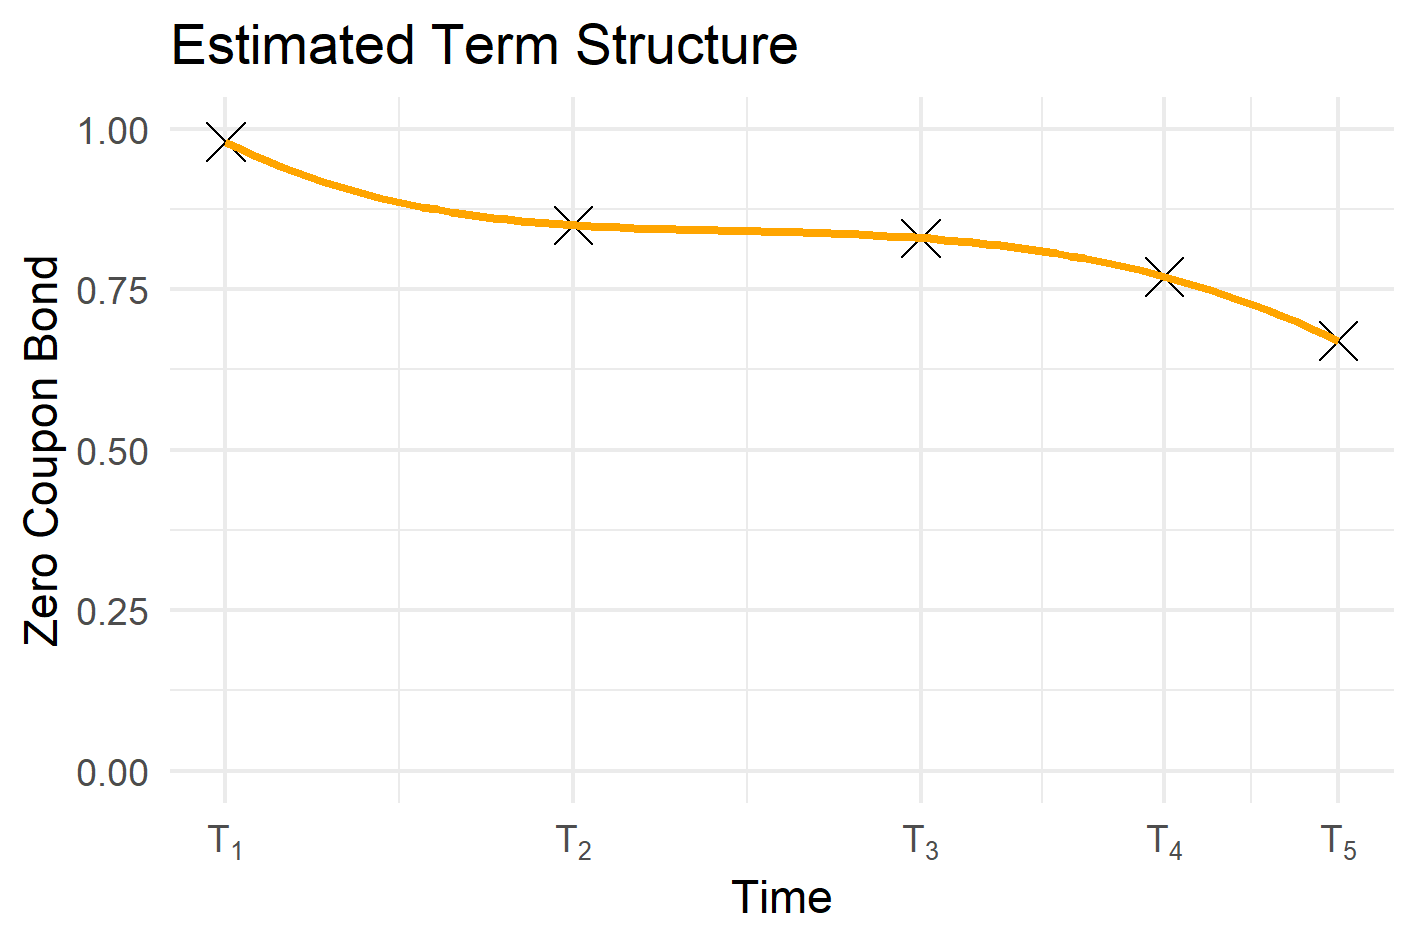
\includegraphics[width=12cm]{figures/Estimating_term_structure.png}
    %\caption{trajectory of ESG-index with underlying process $X(t)$}
    \label{fig: Estimaing_term_structure}
\end{figure}


Typical methods to estimate these term structures are regressions and interpolation methods. We will look at parametric estimation methods, in particular, exponential-polynomial families as these methods are often used by central banks. For instance, the Norwegian Central Bank uses the Svensson method \cite{NB_ZCB}.

\subsection{Exponential-Polynomial Families}
Let $P_{1}, \dots, P_{n}$ be the observed ZCB's with maturities $T_{1}, \dots, T_{n}$, the goal will be the followining: 
\[
\min\limits_{\theta}|P_{\theta}(T_{i}) - P_{i}|^{2}
\]

One proposal is the Nelson-Siegel Curve
\begin{align*}
f_{NS}(T, \underbrace{z_{1}, z_{2}, z_{3}, z_{4}}_{\theta}) 
&= 
z_{1} + (z_{2} + z_{3}T)e^{-z_{4}T}
\end{align*}


where one has the following link between $P_{\theta}$ and $f_{NS}$: 
\begin{align*}
P_{\theta}(T) &= \exp\left(
-\int_{0}^{T}f_{NS}(u;\theta)du
\right)    
\end{align*}

The Svensson curve is given by: 
\begin{align*}
f_{S}(T, \theta) &= 
z_{1} + (z_{2}+z_{3}T)e^{-z_{5}T} + z_{4}Te^{-z_{6}T}
\end{align*}






\newpage 
\section{Forward Measures}
Consider the following probability space $(\Omega, \F, (\F_{t})_{t \in [0,T]}, Q))$, furthermore let $X\in L^{1}(\Omega, \F, Q)$ as well as $\F_{T}$-measurable. The goal of this section is to study: 
\begin{align*}
\pi(t) &= \E_{Q}\left[
\frac{B(t)}{B(T)}X\bigg{|}\F_{t}
\right]    
\end{align*}

\begin{notation}
We use the following notation: 
\begin{align*}
Z^{T}(t) := \frac{P(t,T)}{P(0,T)B(t)}    
\end{align*}
\end{notation}

\begin{proposition}
\label{prop: Z(T)(t)_Q_martingale}
Assume that $\E_{Q}\left[e^{\frac{1}{2}\int_{0}^{T}\norm{v(s,T)}^{2}ds}\right] < \infty \; \forall T$, then we have that: 
\begin{align*}
Z^{T}(t) 
&= \mathcal{E}_{t}(v(\cdot, T)\bullet W^{Q}), \; t\leq T
\end{align*}
is a $Q$-martingale, furthermore there $\exists\; Q^{T}\sim Q$ such that:
\begin{align*}
\frac{dQ^{T}}{dQ}\bigg{|}_{\F_{t}} = Z^{T}(t)    
\end{align*}
and: 
\begin{align*}
dW^{T}(t) = dW^{Q}(t) - v(t,T)dt    
\end{align*}
defines a $Q^{T}$-Brownian motion. 
\end{proposition}

\begin{proof}
Since we assume that $\E_{Q}\left[e^{\frac{1}{2}\int_{0}^{T}\norm{v(s,T)}^{2}ds}\right] < \infty \; \forall T$, it follows from Novikov's condition (\ref{thm: Novikov_cond_and_implications}) and Theorem $\ref{thm: arbitrage_condition_Q}$, that $Z^{T}(t)$ is a $Q$-martingale. Girsanov's Theorem (\ref{thm: Girsanov's_thm}) justifies that  $\exists\; Q^{T}\sim Q$ such that 
$$
\frac{dQ^{T}}{dQ}\bigg{|}_{\F_{t}} = Z^{T}(t)
$$
and that $dW^{T}(t) = dW^{Q}(t) - v(t,T)dt$ defines a $Q^{T}$-Brownain motion. 
\end{proof}


\begin{proposition}[\textbf{\cite{filipovic2009term}}]
\label{prop: general_option_price}
Let $X \in L^{1}(\Omega, \F, Q)$ as well as $\F_{T}$-measurable, we then have that: 
\[
\E_{Q^{T}}[|X|] < \infty
\]
and: 
\begin{align*}
\pi(t) &= P(t,T)\E_{Q^{T}}[X|\F_{t}]    
\end{align*}
\end{proposition}

\begin{proof}
We get from Bayes theorem (\ref{thm: Bayes_thm}) the following: 
\begin{align*}
\E_{Q^{T}}[|X|] &= \frac{
\E_{Q}\left[|X|\frac{dQ^{T}}{dQ}\right]
}{
\E_{Q}\left[\frac{dQ^{T}}{dQ}\right]
} \\ 
&= 
\frac{
\E_{Q}\left[|X|Z^{T}(T)\right]
}{
Z^{T}(0)
} \\ 
&= 
\E_{Q}\left[
\frac{|X|}{P(0,T)B(T)}
\right] \\
&\leq \E_{Q}[|X|] < \infty
\end{align*}

The second part also relies on Bayes theorem: 
\begin{align*}
\E_{Q^{T}}[X|\F_{t}]
&= 
\frac{
\E_{Q}\left[
X\frac{dQ^{T}}{dQ}\bigg{|}\F_{t}
\right]
}{
\E_{Q}\left[
\frac{dQ^{T}}{dQ}\bigg{|}\F_{t}
\right]
} \\ 
&= 
\frac{
\E_{Q}\left[
XZ^{T}(T)\bigg{|}\F_{t}
\right]
}{
Z^{T}(t)
} \\ 
&\Downarrow \\ 
Z^{T}(t)\E_{Q^{T}}[X|\F_{t}] &= \E_{Q}[XZ^{T}(T)|\F_{t}] \\ 
&\Downarrow \\ 
\pi(t):= P(t,T)\E_{Q^{T}}[X|\F_{t}] &= \E_{Q}\left[
\frac{B(t)}{B(T)}X\bigg{|}\F_{t}
\right]
\end{align*}

\end{proof}


\begin{lemma}[\textbf{\cite{filipovic2009term}}]
\label{lemma: T-discounted-S-discounted-bond}
Let $S>0$ and $S\leq T$. Then the $T$-bond discounted $S$-bond price process:
\begin{align*}
\frac{P(t,S)}{P(t,T)}
&= 
\frac{P(0,S)}{P(0,T)}\mathcal{E}_{t}(\sigma_{S,T}\bullet W^{T}), \;\;t\leq S\leq T
\end{align*}
is a $Q^{T}$-martingale. Where we define: 
\begin{align*}
\sigma_{S,T}(t) &= - \sigma_{T,S}(t) = v(t,S) - v(t,T) = \int_{S}^{T}\sigma(t,u)du    
\end{align*}
Moreover, the $T$- and $S$-forward measures are related by: 
\begin{align*}
\frac{dQ^{S}}{dQ^{T}}\bigg{|}_{\F_{t}}
&= 
\frac{P(t,S)}{P(t,T)}\frac{P(0,T)}{P(0,S)} = \mathcal{E}_{t}(\sigma_{S,T}\bullet W^{T})
\end{align*}
\end{lemma}

\begin{proof}
Quite involved, so we start on the next page: 
\newpage 
\textbf{$Q^{T}$-martingality}: 
\\~\\ 
Let $u\leq t \leq S\leq T$, we then get: 
\begin{align*}
\E_{Q^{T}}\left[
\frac{P(t,S)}{P(t,T)}\bigg{|}\F_{u}
\right] 
&\stackrel{\text{Bayes:\ref{thm: Bayes_thm}}}{=}
\underbrace{\frac{
\E_{Q}\left[
\frac{P(t,S)}{P(t,T)}Z^{T}(T)\bigg{|}\F_{u}
\right]
}{
\E_{Q}\left[
Z^{T}(T)|\F_{u}
\right]
}}_{(*)}
\end{align*}
Now from Proposition \ref{prop: Z(T)(t)_Q_martingale} and the Tower law of conditional expectation (Theorem \ref{thm: Tower_law}), we get that: 
\begin{align*}
(*)
&= 
\frac{
\E_{Q}\left[
\E_{Q}\left[\frac{P(t,S)}{P(t,T)}Z^{T}(T)\bigg{|}\F_{t} \right]
\bigg{|}\F_{u}\right]
}{
Z^{T}(u)
} \\ 
&= 
\frac{
\E_{Q}\left[
\frac{P(t,S)}{P(t,T)}\frac{P(t,T)}{P(0,T)B(t)}
\bigg{|}\F_{u}\right]
}{
\frac{P(u,T)}{P(0,T)B(u)}
} \\ 
&= 
\frac{
\E_{Q}\left[
\frac{P(t,S)}{B(t)}
\bigg{|}\F_{u}\right]
}{
\frac{P(u,T)}{B(u)}
}
= \frac{P(u,S)}{P(u,T)}
\end{align*}
Where the last equality comes from the fact that the discounted zero coupon bond process is a $Q$-martingale.
\\~\\ 
\textbf{Explicit expression:}
\\~\\
From Proposition \ref{prop: Z(T)(t)_Q_martingale}, we have that: 
$P(t,T) = B(t)P(0,T)\mathcal{E}_{t}(v(\cdot, T)\bullet W^{Q})$, this yields: 
\begin{align*}
\frac{P(t,S)}{P(t,T)} 
&= 
\frac{P(0,S)}{P(0,T)}
\frac{
\exp\left(
\int_{0}^{t}v(u,S)dW^{Q}(u) - \frac{1}{2}\int_{0}^{t}\norm{v(u,S)}^{2}du
\right)
}{
\exp\left(
\int_{0}^{t}v(u,T)dW^{Q}(u) - \frac{1}{2}\int_{0}^{t}\norm{v(u,T)}^{2}du
\right)
} \\ 
&= 
\frac{P(0,S)}{P(0,T)}
\exp\left(
\underbrace{
\int_{0}^{t}[v(u,S)-v(u,T)]dW^{Q}(u) 
-\frac{1}{2}\int_{0}^{t}\left(
\norm{v(u,S)}^{2} - \norm{v(u,T)}^{2}
\right)du}_{=(*)}
\right)
\end{align*}
Now: $dW^{Q}(u) = dW^{T}(u) + v(u,T)du$, this leaves us with: 
\begin{align*}
(*) &= \int_{0}^{t}[v(u,S)-v(u,T)]dW^{T}(u) 
+ \int_{0}^{t}[v(u,S)-v(u,T)]v(u,T)du 
-\frac{1}{2}
\int_{0}^{t}\left(
\norm{v(u,S)}^{2}-\norm{v(u,T)}^{2}
\right)du
\end{align*}

\newpage 

Now let's collect the $du$-terms into one integral, and work with the inner expression 
\begin{align*}
&[v(u,S)-v(u,T)]v(u,T) -\frac{1}{2}\left(\norm{v(u,S)}^{2}-\norm{v(u,T)}^{2}\right) \\
=& 
v(u,S)v(u,T)-\norm{v(u,T)}^{2} -\frac{1}{2}\norm{v(u,S)}^{2} + \frac{1}{2}\norm{v(u,T)}^{2} \\ 
=& 
v(u,S)v(u,T)-\frac{1}{2}\norm{v(u,T)}^{2} - \frac{1}{2}\norm{v(u,S)}^{2} \\ 
=& 
-\frac{1}{2}\norm{v(u,S)-v(u,T)}^{2} \\ 
=& -\frac{1}{2}\norm{\sigma_{S,T}(u)}^{2}
\end{align*}
Thus: 
\begin{align*}
\frac{P(t,S)}{P(t,T)}
&= 
\frac{P(0,S)}{P(0,T)}\exp\left(
\int_{0}^{t}\sigma_{S,T}(u)dW^{T}(u) -\frac{1}{2}\int_{0}^{t}\norm{\sigma_{S,T}(u)}^{2}du 
\right) \\ 
&= 
\frac{P(0,S)}{P(0,T)}\mathcal{E}_{t}\left(
\sigma_{S,T}\bullet W^{T}
\right)
\end{align*}

\textbf{Radon-Nikodym derivative:}
\\~\\ 
We have that: 
\begin{align*}
\frac{dQ^{S}}{dQ^{T}}\bigg{|}_{\F_{t}} 
&= 
\frac{dQ^{S}}{dQ}\bigg{|}_{\F_{t}}\bullet\left(
\frac{dQ^{T}}{dQ}\bigg{|}_{\F_{t}}
\right)^{-1} \\ 
&= 
Z^{S}(t)[Z^{T}(t)]^{-1} \\ 
&= 
\frac{P(t,S)}{P(0,S)B(t)}\frac{P(0,T)B(t)}{P(t,T)} \\ 
&= 
\frac{
P(t,S)P(0,T)
}{
P(t,T)P(0,S)
} \\ 
&= 
\mathcal{E}_{t}\left(
\sigma_{S,T}\bullet W^{T}
\right)
\end{align*}
\end{proof}

\newpage 
\section{The LIBOR market model}

In a \textbf{Market model} one is interested in modelling only the relevant $T$'s, meaning that one finds a model for each $T_{i}$. In the market, there are essentially three types of interest rate derivatives: \textbf{caps}, \textbf{floors} and 
\textbf{swaptions}. By swaption, we mean a call/put on a swap.

\begin{definition}[\textbf{LIBOR-rate}]
 We define the LIBOR-rate $L(t,T)$ as: 
 \begin{align*}
L(t,T) &= F(t,T,T+\delta) 
= \frac{1}{\delta}\left(
\frac{P(t,T)}{P(t,T+\delta)}-1
\right)     
 \end{align*}
\end{definition}

\begin{definition}[\textbf{LIBOR-Caplet}]
A caplet with reset date \textbf{T} and settlement \textbf{T+$\delta$} pays the holder: LIBOR minus strike $\kappa$ if it is positive: 
\begin{align*}
\delta(F(T;T,T+\delta) -\kappa)^{+} = \delta(L(T,T)-\kappa)^{+}
\end{align*}
\end{definition} 

\begin{definition}[\textbf{LIBOR-Floorlet}]
The opposite of a caplet, it has the following payoff: 
\begin{align*}
\delta(\kappa - L(T,T))^{+}    
\end{align*}
\end{definition}

We assume equidistant times $T_{m} = m\delta, m = 0, 1, \dots, M$, furthermore we will work on: 
$(\Omega, \F, (\F_{t})_{t\in [0,T_{M}]}, Q^{T_{M}})$, $W^{T_{M}}(t)$ is a $Q^{T_{M}}$-BM. In addition $L(0,T_{i})\geq 0 $ are given for $m = 1, \dots, M-1$: 
\begin{align*}
L(0,T_{m}) &= \frac{1}{\delta}\left(
\frac{P(0,T_{m})}{P(0,T_{m+1})}-1
\right), \;\; m = 0, \dots, M-1   
\end{align*}

We get the following timeline:

\begin{tikzpicture}[snake=zigzag, line before snake = 5mm, line after snake = 5mm]
    % draw horizontal line   
    \draw (0,0) -- (2,0);
    \draw[snake] (2,0) -- (4,0);
    \draw (4,0) -- (5,0);
    \draw[snake] (5,0) -- (7,0);
    %\draw[snake] (7,0) -- (9,0);
    \draw (7,0) -- (9,0);

    % draw vertical lines
    \foreach \x in {0,1,2,4,5,7,8}
      \draw (\x cm,3pt) -- (\x cm,-3pt);

    % draw nodes
    \draw (0,0) node[below=3pt] {$ t $} node[above=3pt] {$   $};
    \draw (1,0) node[below=3pt] {$ T_{m} $} node[above=3pt] {$  $};
    \draw (2,0) node[below=3pt] {$ T_{m+1} $} node[above=3pt] {$  $};
    \draw (3,0) node[below=3pt] {$  $} node[above=3pt] {$  $};
    \draw (4,0) node[below=3pt] {$ T_{n} $} node[above=3pt] {$  $};
    \draw (5,0) node[below=3pt] {$ T_{n+1} $} node[above=3pt] {$  $};
    \draw (6,0) node[below=3pt] {$  $} node[above=3pt] {$  $};
    \draw (7,0) node[below=3pt] {$ T_{M-1} $} node[above=3pt] {$ $};
    \draw (8,0) node[below=3pt] {$ T_{M} $} node[above=3pt] {$ $};
  \end{tikzpicture}



The dynamics of $L(t,T_{M-1})$ are given by: 
\begin{align*}
dL(t,T_{M-1}) &= L(t,T_{M-1})\lambda(t,T_{M-1})dW^{T_{M}}(t), \;\; t \leq T_{M-1} \\ 
&\Downarrow \\ 
L(t,T_{M-1}) &= L(0,T_{M-1})\exp\left(
\int_{0}^{t}\lambda(s,T_{M-1})dW^{T_{M}}(s) 
-\frac{1}{2}\int_{0}^{t}\norm{\lambda(s, T_{M-1})}^{2}ds
\right)
\end{align*}

Here: $t \mapsto \lambda(t,T_{M-1})$ is assumed to be an $\R^{d}$-valued bounded deterministic measurable function. 
\\~\\ 
Since
\begin{align*}
\E_{Q^{T_{M}}}\left[
e^{\frac{1}{2}\int_{0}^{T_{M-1}}\norm{\lambda(s,T_{M-1}}ds}
\right] < \infty 
\;\;\text{and}\;\;
\frac{L(t,T_{M-1})}{L(0,T_{M-1})} = \mathcal{E}_{t}\left(
\lambda(\cdot, T_{M-1})\bullet W^{T_{M}})
\right)
\end{align*}

We have that $L(t,T_{M-1})$ is a $Q^{T_{M}}$-martingale. The idea will be to iterate backwards, so that $L(t,T_{m-1})$ will be martingales under $Q^{T_{m}}$ for $m\geq 2$, we thus need valid measure changes from $Q^{T_{m}}$ to $Q^{T_{m-1}}$ on $\F_{T_{m-1}}$

\newpage

One defines:
\begin{align*}
\frac{
dQ^{T_{M-1}}
}{
dQ^{T_{M}}
}\bigg{|}_{\F_{T_{M-1}}}
&= 
\mathcal{E}_{T_{M-1}}\left(
\sigma_{T_{M-1}, T_{M}}\bullet W^{T_{M}}
\right)
\end{align*}

Where: 
\begin{align*}
\sigma_{T_{M-1}, T_{M}}(t) := 
\frac{
\delta L(t,T_{M-1})
}{
\delta L(t,T_{M-1}) + 1
}
\lambda(t,T_{M-1}), \;t\leq T_{M-1}
\end{align*}

Let $K\in \R$, now as: 
\begin{align*}
\norm{\sigma_{T_{M-1}, T_{M}}(t)}^{2}
&\leq 
\norm{\lambda(t,T_{M-1})}^{2} \leq K \\ 
&\Downarrow \\ 
\E_{Q^{T_{M}}}\left[
e^{
\frac{1}{2}\int_{0}^{T_{M-1}}\norm{\sigma_{T_{M-1}, T_{M}}(s)}^{2}ds
}
\right]
&\leq 
e^{
\frac{1}{2}T_{M-1}K
} < \infty
\end{align*}


Furthermore: 
\begin{align*}
\E_{Q^{T_{M}}}\left[
\frac{
dQ^{T_{M-1}}
}{
dQ^{T_{M}}
}\bigg{|}_{\F_{T_{M-1}}}
\right] 
&= 
\E_{Q^{T_{M}}}\left[
\frac{
dQ^{T_{M-1}}
}{
dQ^{T_{M}}
}\bigg{|}_{\F_{T_{M-1}}}
\bigg{|}\F_{0}
\right] 
=  
\mathcal{E}_{0}\left(
\sigma_{T_{M-1}, T_{M}} \bullet W^{T_{M}}
\right)
= 1
\end{align*}

We thus have that $Q^{T_{M-1}} \sim Q^{T_{M}}$ and from Girsanov's Theorem we have that: 
\begin{align*}
dW^{T_{M-1}}(t) = dW^{T_{M}}(t) - \sigma_{T_{M-1}, T_{M}}(t)dt   
\end{align*}

defines a Brownian Motion on $Q^{T_{M-1}}$. 

\begin{lemma}[\textbf{\cite{filipovic2009term}}]
Let $X$ be a $T_{m}$-contingent claim, we then have that for \\ $t\leq T_{m} \leq T_{n}$ 
\begin{align*}
\frac{\pi(t)}{P(t,T_{m})} 
&= 
\frac{
P(t,T_{n})
}{
P(t,T_{m})
}\E_{Q^{T_{n}}}\left[
\frac{X}{P(T_{m}, T_{n})}
\bigg{|}\F_{t}
\right]
\end{align*}
\end{lemma} 

\begin{proof}
We already have that $\pi(t) = P(t,T_{m})\E_{Q^{T_{m}}}[X|\F_{t}]$, and from 
Lemma \ref{lemma: T-discounted-S-discounted-bond}, by using $S = T_{n}$ and $T = T_{m}$, we have:
\begin{align*}
\frac{
dQ^{T_{m}}
}{
dQ^{T_{n}}
}\bigg{|}_{\F_{t}}
&= 
\mathcal{E}_{t}\left(
\sigma_{T_{m}, T_{n}}\bullet W^{T_{n}}
\right)
\end{align*}

This is a $Q^{T_{n}}$-martingale, now in combination with Bayes Theorem, we get: 
\begin{align*}
\E_{Q^{T_{m}}}\left[
X|\F_{t}
\right]
&= 
\frac{
\E_{Q^{T_{n}}}\left[
\frac{P(T_{m}, T_{m})}{P(T_{m}, T_{n})}
\frac{P(0, T_{n})}{P(0, T_{m})}
\bigg{|}\F_{t}\right]
}{
\frac{P(t, T_{m})}{P(t, T_{n})}
\frac{P(0, T_{n})}{P(0, T_{m})}
} \\ 
&= 
\frac{P(t, T_{n})}{P(t, T_{m})}
\E_{Q^{T_{n}}}\left[
\frac{X}{P(T_{m}, T_{n})}
\bigg{|}\F_{t}\right]
\end{align*}

\end{proof}


